%%%%%%%%%%%%%%%%%%%%%%%%%%%%%%%%%%%%%%%%%
% Beamer Presentation - LaTeX Template
% Version 2.0 (March 8, 2022)
% Original Template: https://www.LaTeXTemplates.com
% Author: Vel (vel@latextemplates.com)
% License: CC BY-NC-SA 4.0

% Este modelo de apresentação foi 
% criado a partir do modelo de Giovanni Spadaro.
% Disponível em: https://github.com/Giovo17/presentation-template-unict-lm-data
%
% Adaptado por Lucas Amaral Taylor para criar uma versão especial 
% para os alunos de Matemática e Estatística da USP (IME-USP).
% Disponível em: https://github.com/lucasamtaylor01/IME-template
%%%%%%%%%%%%%%%%%%%%%%%%%%%%%%%%%%%%%%%%%

%----------------------------------------------------------------------------------------
% CLASSE DO DOCUMENTO E CONFIGURAÇÕES BÁSICAS
%----------------------------------------------------------------------------------------
\documentclass[
    11pt,               % Tamanho padrão da fonte
    % t,                % Alinhar verticalmente ao topo
    %aspectratio=169,   % Definir proporção 16:9
]{beamer}
\graphicspath{{img/}}         % Define o diretório das imagens

%----------------------------------------------------------------------------------------
% PACOTES NECESSÁRIOS
%----------------------------------------------------------------------------------------
\usepackage{
    booktabs,     % Melhora a aparência das linhas em tabelas
    palatino,     % Define Palatino como fonte principal
    subcaption    % Suporte para subfiguras
}
\usepackage[default]{opensans}  % Define Open Sans como fonte secundária
%----------------------------------------------------------------------------------------
%	PACOTES E CONFIGURAÇÕES PARA CÓDIGO
%----------------------------------------------------------------------------------------
% Pacotes necessários para formatação de código
\usepackage[utf8]{inputenc}
\usepackage{listings}
\usepackage{xcolor}

% Cores para syntax highlighting (VSCode Light Theme)
\definecolor{vscBackground}{RGB}{255,255,255}    % Fundo branco
\definecolor{vscKeyword}{RGB}{175,0,219}         % Roxo para palavras-chave
\definecolor{vscString}{RGB}{163,21,21}          % Vermelho para strings
\definecolor{vscComment}{RGB}{0,128,0}           % Verde para comentários
\definecolor{vscFunction}{RGB}{121,94,38}        % Marrom para funções
\definecolor{vscNumber}{RGB}{9,134,88}           % Verde escuro para números
\definecolor{vscOperator}{RGB}{175,0,219}        % Roxo para operadores
\definecolor{vscText}{RGB}{0,0,0}                % Texto preto
\definecolor{vscLineNr}{RGB}{128,128,128}        % Cinza para números de linha

% Configuração geral do listings para UTF-8
\lstset{
    inputencoding=utf8,
    extendedchars=true,
    literate=%
        {á}{{\'a}}1 {é}{{\'e}}1 {í}{{\'i}}1 {ó}{{\'o}}1 {ú}{{\'u}}1
        {Á}{{\'A}}1 {É}{{\'E}}1 {Í}{{\'I}}1 {Ó}{{\'O}}1 {Ú}{{\'U}}1
        {à}{{\`a}}1 {è}{{\`e}}1 {ì}{{\`i}}1 {ò}{{\`o}}1 {ù}{{\`u}}1
        {À}{{\`A}}1 {È}{{\'E}}1 {Ì}{{\`I}}1 {Ò}{{\`O}}1 {Ù}{{\`U}}1
        {ã}{{\~a}}1 {ẽ}{{\~e}}1 {ĩ}{{\~i}}1 {õ}{{\~o}}1 {ũ}{{\~u}}1
        {Ã}{{\~A}}1 {Ẽ}{{\~E}}1 {Ĩ}{{\~I}}1 {Õ}{{\~O}}1 {Ũ}{{\~U}}1
        {â}{{\^a}}1 {ê}{{\^e}}1 {î}{{\^i}}1 {ô}{{\^o}}1 {û}{{\^u}}1
        {Â}{{\^A}}1 {Ê}{{\^E}}1 {Î}{{\^I}}1 {Ô}{{\^O}}1 {Û}{{\^U}}1
        {ç}{{\c c}}1 {Ç}{{\c C}}1
        {º}{{\textordmasculine}}1
        {ª}{{\textordfeminine}}1
}

% Configurações base comum para todas as linguagens
\lstdefinestyle{baseStyle}{
    backgroundcolor=\color{vscBackground},
    basicstyle=\ttfamily\small\color{vscText},
    breakatwhitespace=false,
    breaklines=true,
    captionpos=b,
    keepspaces=true,
    numbers=left,
    numbersep=5pt,
    showspaces=false,
    showstringspaces=false,
    showtabs=false,
    tabsize=4,
    frame=single,
    framerule=0.8pt,
    rulecolor=\color{gray!20},
    numberstyle=\tiny\color{vscLineNr},
    keywordstyle=\color{vscKeyword},
    commentstyle=\color{vscComment}\itshape,
    stringstyle=\color{vscString},
    emphstyle=\color{vscFunction},
    columns=flexible,
    basewidth={0.5em,0.45em},
    inputencoding=utf8,
    extendedchars=true
}

%----------------------------------------------------------------------------------------
% Python
%----------------------------------------------------------------------------------------
\lstdefinestyle{pythonStyle}{
    style=baseStyle,
    language=Python,
    morekeywords={self,None,True,False,import,from,as,def,class,return,yield,
                  for,while,if,else,elif,try,except,finally,with,lambda,
                  async,await,break,continue,global,nonlocal,pass,raise},
    morekeywords=[2]{print,len,range,type,int,str,float,list,dict,set,
                     tuple,max,min,sum,sorted,enumerate,zip,map,filter,
                     any,all,abs,round,pow,divmod},
    keywordstyle=[2]\color{vscFunction},
    sensitive=true
}

\lstnewenvironment{python}[1][]{\lstset{style=pythonStyle, #1}}{}
\newcommand{\pyinline}[1]{\lstinline[style=pythonStyle]!#1!}
\newcommand{\inputpython}[2][]{\lstinputlisting[style=pythonStyle,#1]{#2}}

%----------------------------------------------------------------------------------------
% C Language
%----------------------------------------------------------------------------------------
\lstdefinestyle{cStyle}{
    style=baseStyle,
    language=C,
    morekeywords={include,define,void,int,char,float,double,long,unsigned,
                  struct,union,enum,typedef,const,static,extern,register,
                  auto,volatile,sizeof,return,if,else,for,while,do,switch,
                  case,break,continue,default,goto},
    morekeywords=[2]{printf,scanf,malloc,free,calloc,realloc,fopen,fclose,
                     fprintf,fscanf,strcpy,strlen,strcat},
    keywordstyle=[2]\color{vscFunction},
    sensitive=true
}

\lstnewenvironment{clang}[1][]{\lstset{style=cStyle, #1}}{}
\newcommand{\clinline}[1]{\lstinline[style=cStyle]!#1!}
\newcommand{\inputclang}[2][]{\lstinputlisting[style=cStyle,#1]{#2}}

%----------------------------------------------------------------------------------------
% C++
%----------------------------------------------------------------------------------------
\lstdefinestyle{cppStyle}{
    style=baseStyle,
    language=C++,
    morekeywords={class,private,protected,public,template,typename,namespace,
                  using,new,delete,this,friend,virtual,override,final,explicit,
                  mutable,constexpr,nullptr,noexcept,static_cast,dynamic_cast,
                  const_cast},
    morekeywords=[2]{cout,cin,endl,vector,string,map,set,queue,stack,pair,
                     begin,end,push_back,pop_back,emplace_back,size,empty},
    keywordstyle=[2]\color{vscFunction},
    sensitive=true
}

\lstnewenvironment{cpp}[1][]{\lstset{style=cppStyle, #1}}{}
\newcommand{\cppinline}[1]{\lstinline[style=cppStyle]!#1!}
\newcommand{\inputcpp}[2][]{\lstinputlisting[style=cppStyle,#1]{#2}}

%----------------------------------------------------------------------------------------
% R Language
%----------------------------------------------------------------------------------------
\lstdefinestyle{rStyle}{
    style=baseStyle,
    language=R,
    morekeywords={if,else,repeat,while,function,for,in,next,break,TRUE,FALSE,
                  NULL,Inf,NaN,NA,NA_integer_,NA_real_,NA_complex_,NA_character_},
    morekeywords=[2]{library,require,attach,detach,source,setwd,options,
                     data.frame,read.csv,write.csv,list,matrix,array},
    keywordstyle=[2]\color{vscFunction},
    sensitive=true
}

\lstnewenvironment{rlang}[1][]{\lstset{style=rStyle, #1}}{}
\newcommand{\rlinline}[1]{\lstinline[style=rStyle]!#1!}
\newcommand{\inputrlang}[2][]{\lstinputlisting[style=rStyle,#1]{#2}}

%----------------------------------------------------------------------------------------
% Java
%----------------------------------------------------------------------------------------
\lstdefinestyle{javaStyle}{
    style=baseStyle,
    language=Java,
    morekeywords={abstract,assert,boolean,break,byte,case,catch,char,class,
                  const,continue,default,do,double,else,enum,extends,final,
                  finally,float,for,if,implements,import,instanceof,int,
                  interface,long,native,new,package,private,protected,public,
                  return,short,static,strictfp,super,switch,synchronized,this,
                  throw,throws,transient,try,void,volatile,while},
    morekeywords=[2]{String,System,out,println,printStackTrace,ArrayList,
                     HashMap,Arrays,List,Map,Set,Exception,RuntimeException},
    keywordstyle=[2]\color{vscFunction},
    sensitive=true
}

\lstnewenvironment{java}[1][]{\lstset{style=javaStyle, #1}}{}
\newcommand{\javainline}[1]{\lstinline[style=javaStyle]!#1!}
\newcommand{\inputjava}[2][]{\lstinputlisting[style=javaStyle,#1]{#2}}       % Importa configurações para highlight de código
\usepackage{algorithmicx}
\usepackage{float}

%----------------------------------------------------------------------------------------
% CONFIGURAÇÃO DO TEMA
%----------------------------------------------------------------------------------------
% Tema Base
\usetheme{Boadilla}                          % Define o tema principal
\useinnertheme{circles}                      % Tema interno com círculos
\useoutertheme{miniframes}                   % Tema externo com miniframes
\setbeamertemplate{navigation symbols}{}     % Remove símbolos de navegação

% Cores Personalizadas
\definecolor{primaryColor}{RGB}{20,45,105}   % Cor primária - azul escuro
\definecolor{secondaryColor}{RGB}{0,100,160} % Cor secundária - azul médio

% Configurações de Cores
\setbeamercolor{structure}{fg=primaryColor}
\setbeamercolor{palette primary}{bg=primaryColor, fg=white}
\setbeamercolor{palette secondary}{bg=secondaryColor, fg=white}
\setbeamercolor{title}{bg=primaryColor, fg=white}

% Cores do Cabeçalho e Rodapé
\setbeamercolor{headline}{bg=secondaryColor, fg=white}
\setbeamercolor{section in head/foot}{bg=primaryColor, fg=white}
\setbeamercolor{subsection in head/foot}{bg=secondaryColor, fg=white}
\setbeamercolor{author in head/foot}{bg=primaryColor, fg=white}
\setbeamercolor{title in head/foot}{bg=secondaryColor, fg=white}
\setbeamercolor{date in head/foot}{bg=primaryColor, fg=white}
\setbeamercolor{page number in head/foot}{bg=primaryColor, fg=white}

%----------------------------------------------------------------------------------------
% BIBLIOGRAFIA
%----------------------------------------------------------------------------------------
\usepackage[style=alphabetic,backend=biber]{biblatex}
\addbibresource{bibliografia.bib}

%----------------------------------------------------------------------------------------
% INFORMAÇÕES DA APRESENTAÇÃO
%----------------------------------------------------------------------------------------
\setbeamerfont{title}{size=\small}
\title[]{IA Neurossimbólica para RAG sobre
	Modelos Metabólicos em Escala Genômica: um Estudo
	Comparativo entre RAG Vetorial, GraphRAG e OG-RAG}          % [Versão curta]{Versão completa}
\author[Giovani Tavares]{Giovani Tavares de Andrade}            % [Versão curta]{Nome completo}
\institute[IME-USP]{Instituto de Matemática e Estatística \\ (IME-USP)}
\date[2026]{08 / 2026}

%----------------------------------------------------------------------------------------
% INÍCIO DO DOCUMENTO
%----------------------------------------------------------------------------------------
\begin{document}

% Slide de título com logo
\begin{frame}
	\vspace{-0.5em}
    \begin{figure}
        
\includegraphics[width=0.45\linewidth]{img/logo_IME.png}
    \vspace{-1.5em}
    \end{figure}
    \titlepage
\end{frame}

% Inclusão das seções
\section{\textit{Retrieval Augmented Generation} (RAG)} % Seções são adicionadas para organizar sua apresentação em blocos discretos, todas as seções e subseções são automaticamente exibidas no índice como uma visão geral da apresentação, mas NÃO são exibidas como slides separados.
%----------------------------------------------------------------------------------------
\begin{frame}
	\frametitle{\textit{Retrieval Augmented Generation} (RAG)}
	{\footnotesize
		\begin{itemize}
			\item RAG é uma técnica que combina  LLMs com sistemas de \textbf{recuperação de informação }
			\item  A recuperação de informação (\textit{retrieval}) realiza uma busca dos \textbf{documentos pertinentes} à \textit{query} de modo que eles sejam combinados para formar o \textit{input} do LLM
			\item Fixado o LLM utilizado no sistema, a pertinência dos documentos à \textit{query} está diretamente relacionada à qualidade do \textit{output} gerado pelo RAG
		\end{itemize}
	}
	\begin{figure}[H]
		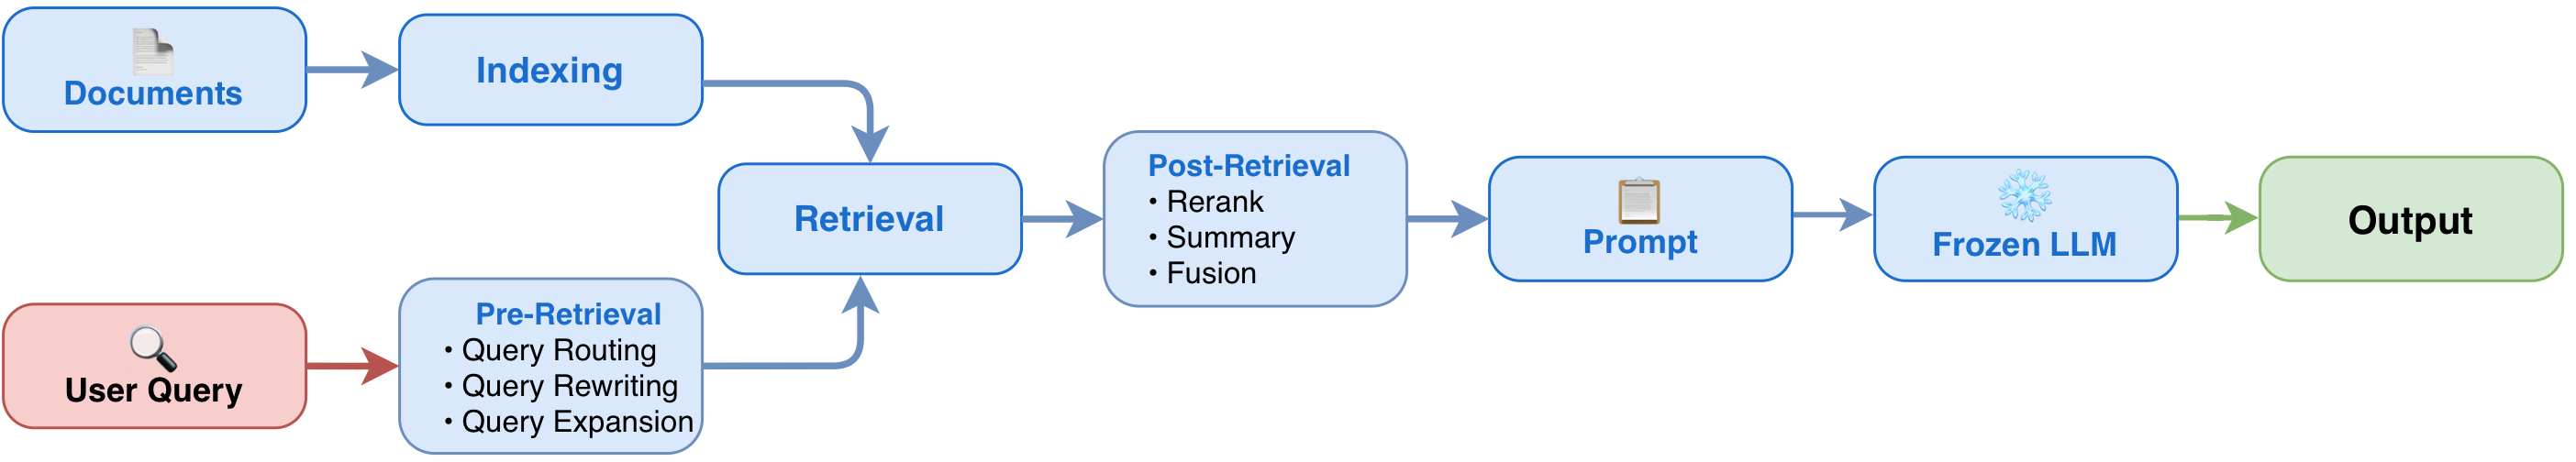
\includegraphics[width=0.85\linewidth]{img/rag_arch.png}
	\end{figure}
\end{frame}
%----------------------------------------------------------------------------------------
\begin{frame}
	\frametitle{Seleção de Documentos Pertinentes}
	\begin{columns}
		\begin{column}{0.50\textwidth}
			{\footnotesize
				\begin{itemize}
					\item A escolha de documentos relevantes à \textit{query} é de responsabilidade da etapa de busca
					\item A \textbf{similaridade de cosseno} é a técnica comumente utilizada para definir relevância
					\item O mesmo modelo de \textit{embeddings} utilizado para gerar os vetores dos \textit{chunks} é utilizado para gerar um vetor da \textit{query}, o que habilita o sistema a utilizar o produto interno entre \textit{chunks} e \textit{query}
				\end{itemize} 
			}
		\end{column}
		\begin{column}{0.40\textwidth}
			\begin{figure}[H]
				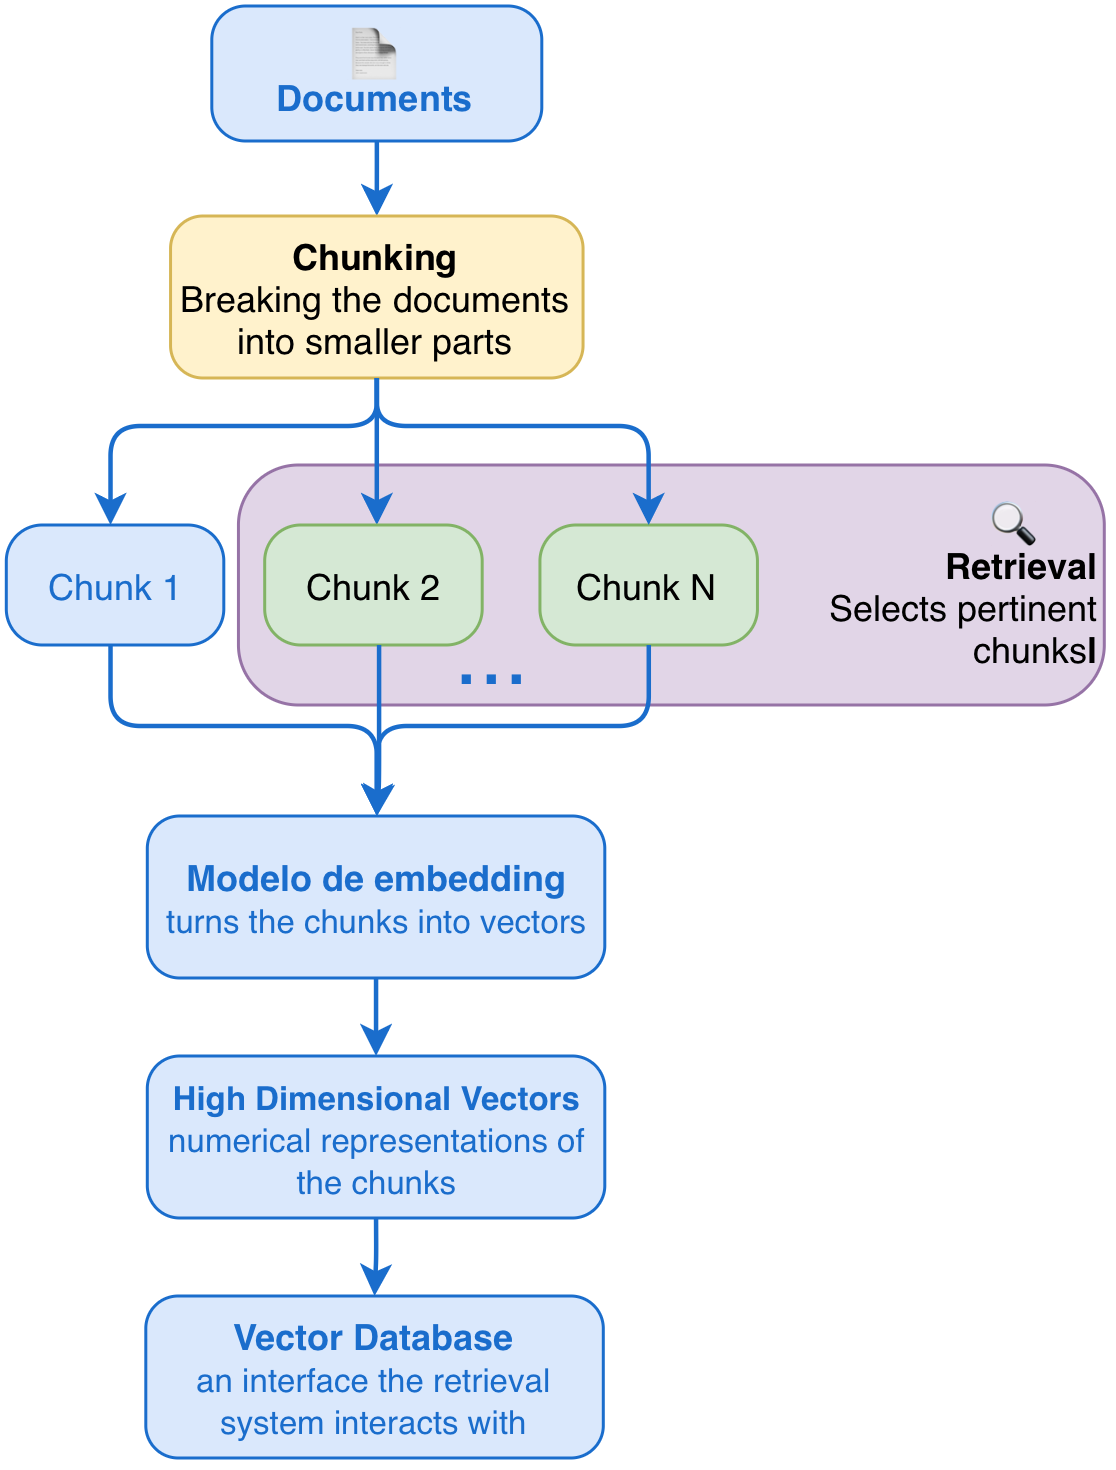
\includegraphics[width=\linewidth]{img/pertinent_chunks_selection.png}
			\end{figure}
		\end{column}
	\end{columns}
\end{frame}
%----------------------------------------------------------------------------------------
\begin{frame}
	\frametitle{Problemas com a Busca Vetorial Pura}
	{\footnotesize
		\begin{itemize}
			\item Seleção de documentos irrelevantes à \textit{query}
			\item Seleção de documentos contraditórios ao conhecimento de domínio
			\item Menor correção atribuída aos \textit{outputs} gerados pelo LLM
			\item Baixa explicabilidade
		\end{itemize}
	}
	
	\begin{figure}[H]
		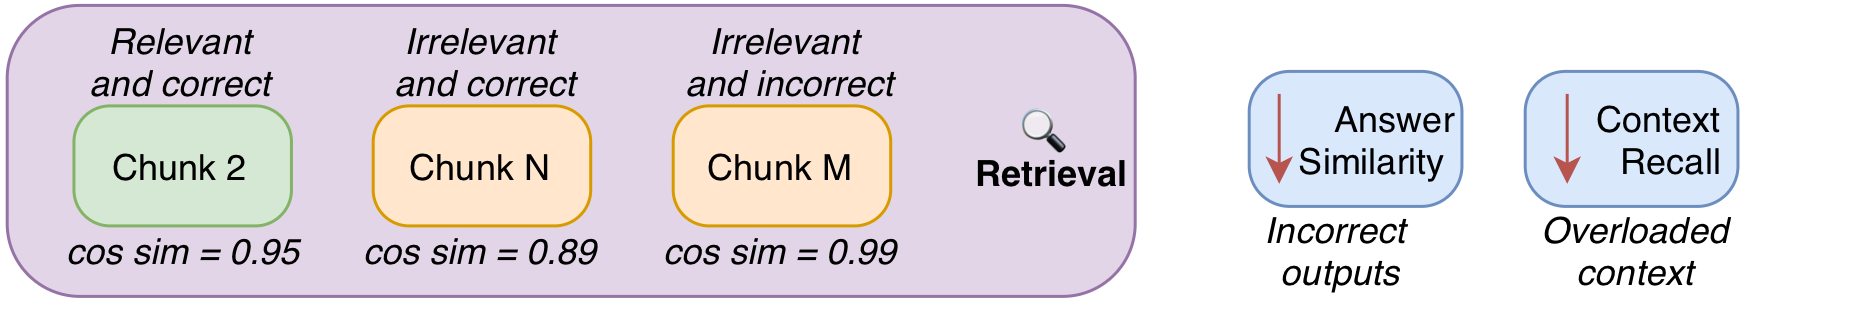
\includegraphics[width=0.85\linewidth]{img/cos_sim_problems.png}
	\end{figure}
	
\end{frame}
%---------------

%---------------------------------------------------------------------------------------- % O que é RAG
\section{Alternativas Neurossimbólicas} % Seções são adicionadas para organizar sua apresentação em blocos discretos, todas as seções e subseções são automaticamente exibidas no índice como uma visão geral da apresentação, mas NÃO são exibidas como slides separados.

\begin{frame}
	\frametitle{OG-RAG}
	{\footnotesize
		\begin{itemize}
			\item O OG-RAG é uma arquitetura que adiciona uma \textbf{ontologia curada por humanos} ao processo de \textit{chunking} dos documentos de domínio  representado nos documentos
			\item Uma \textit{ontologia} é uma representação simbólica do conhecimento do domínio representado nos documentos
			\item  A \textbf{ontologia} é curada por especialistas do domínio e permite que cada \textit{chunk} carregue a semântica formal do conhecimento representado nos documentos
		\end{itemize}
	}
	\begin{figure}[H]
		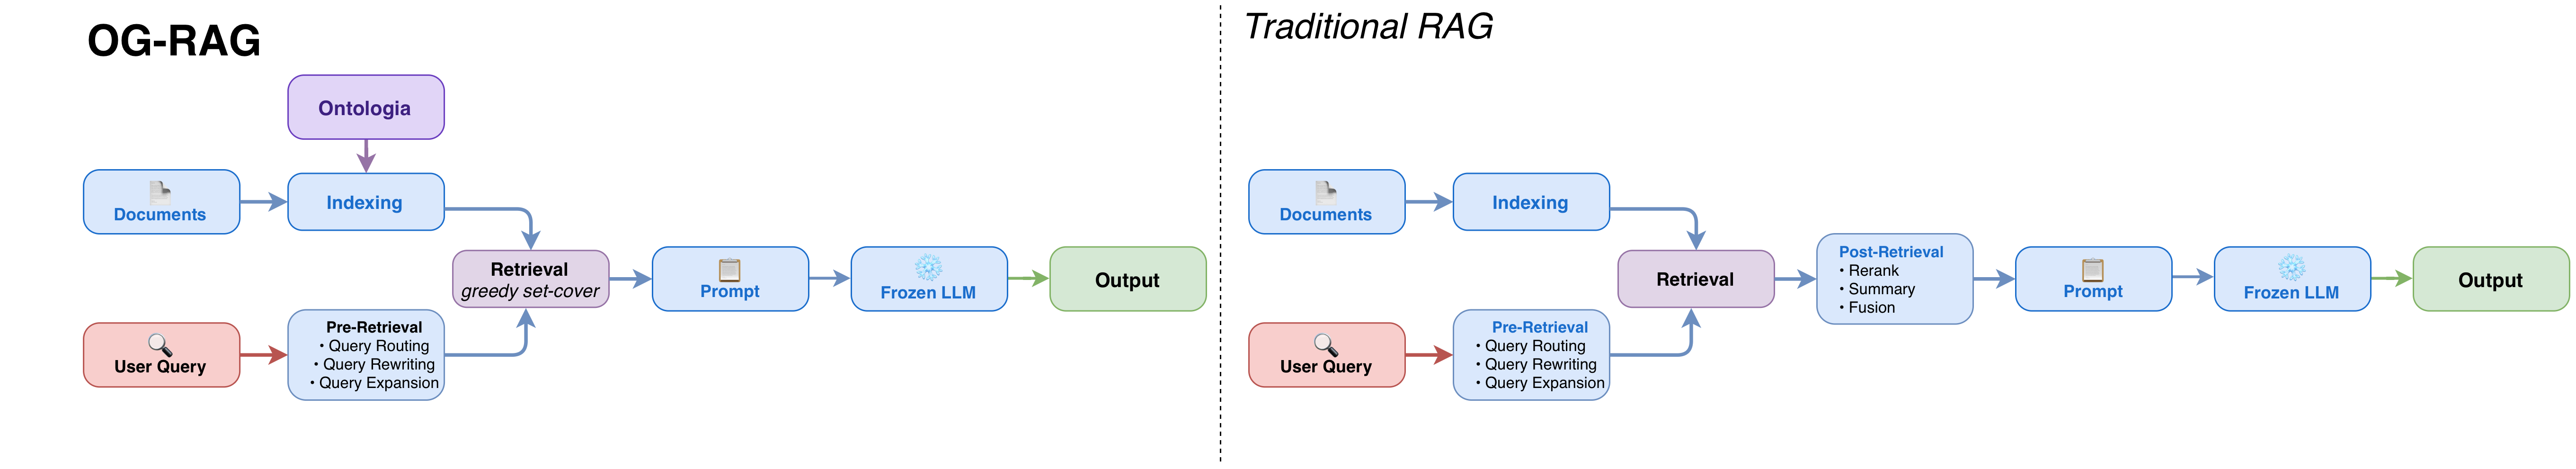
\includegraphics[width=1.0\linewidth]{img/og_rag_vs_trad_rag.png}
	\end{figure}
\end{frame}

\begin{frame}
	\frametitle{GraphRAG}
	{\footnotesize
		\begin{itemize}
			\item O GraphRAG é uma arquitetura que, na indexação, usa um \textbf{LLM} para extrair \textbf{entidades e relações} dos documentos, construindo um \textbf{grafo de conhecimento sintético}
			\item As entidades são agrupadas em \textbf{comunidades}, e o LLM gera um \textit{community report} (resumo) para cada uma
			\item O \textit{retrieval} assume duas formas: \textbf{\textit{Local Search}}, que percorre o grafo a partir das entidades extraídas da \textit{query}, e \textbf{\textit{Global Search}}, que agrega os \textit{community reports} via \textbf{Map-Reduce}
		\end{itemize}
	}
	\begin{figure}[H]
		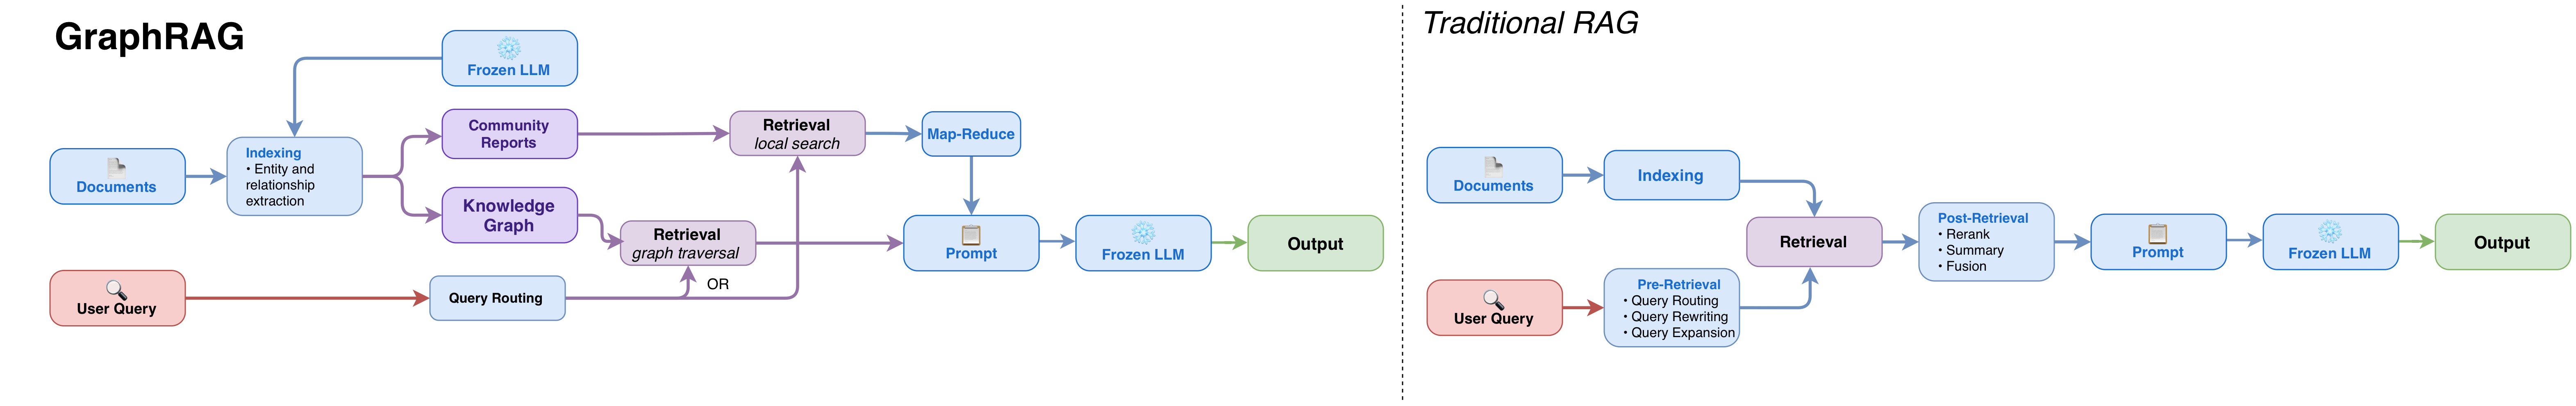
\includegraphics[width=1.0\linewidth]{img/graphrag_vs_trad_rag.png}
	\end{figure}
\end{frame} % O que é o RAG com busca vetorial 
\section{OntoGEM} % Seções são adicionadas para organizar sua apresentação em blocos discretos, todas as seções e subseções são automaticamente exibidas no índice como uma visão geral da apresentação, mas NÃO são exibidas como slides separados.

%----------------------------------------------------------------------------------------
%----------------------------------------------------------------------------------------

\begin{frame}{OntoGEM}
	\begin{itemize}
		\item O processo de construção de um modelo computacional do metabolismo de um organismo é conhecido
		como \textbf{reconstrução}, enquanto o modelo resultante é frequentemente denominado \textbf{modelo metabólico em
			escala genômica (GEM)}.
		\item Durante o processo de reconstrução, especialistas do domínio precisam revisar diferentes banco de dados e a literatura respondendo perguntas como:
		\begin{itemize}
			\item \textit{Quais são os substratos da reação \textbf{R}}?
			\item \textit{Quais representações alternativas existem para a reação \textbf{R}?}
		\end{itemize}
		\item  Souza, N. A. de (2025) construiu a ontologia OntoGEM com o apoio de especialistas de domínio para facilitar o processo de reconstrução e de resolução das perguntas
	\end{itemize}     
\end{frame}

%----------------------------------------------------------------------------------------

\begin{frame}{OntoGEM}
	\begin{figure}[H]
		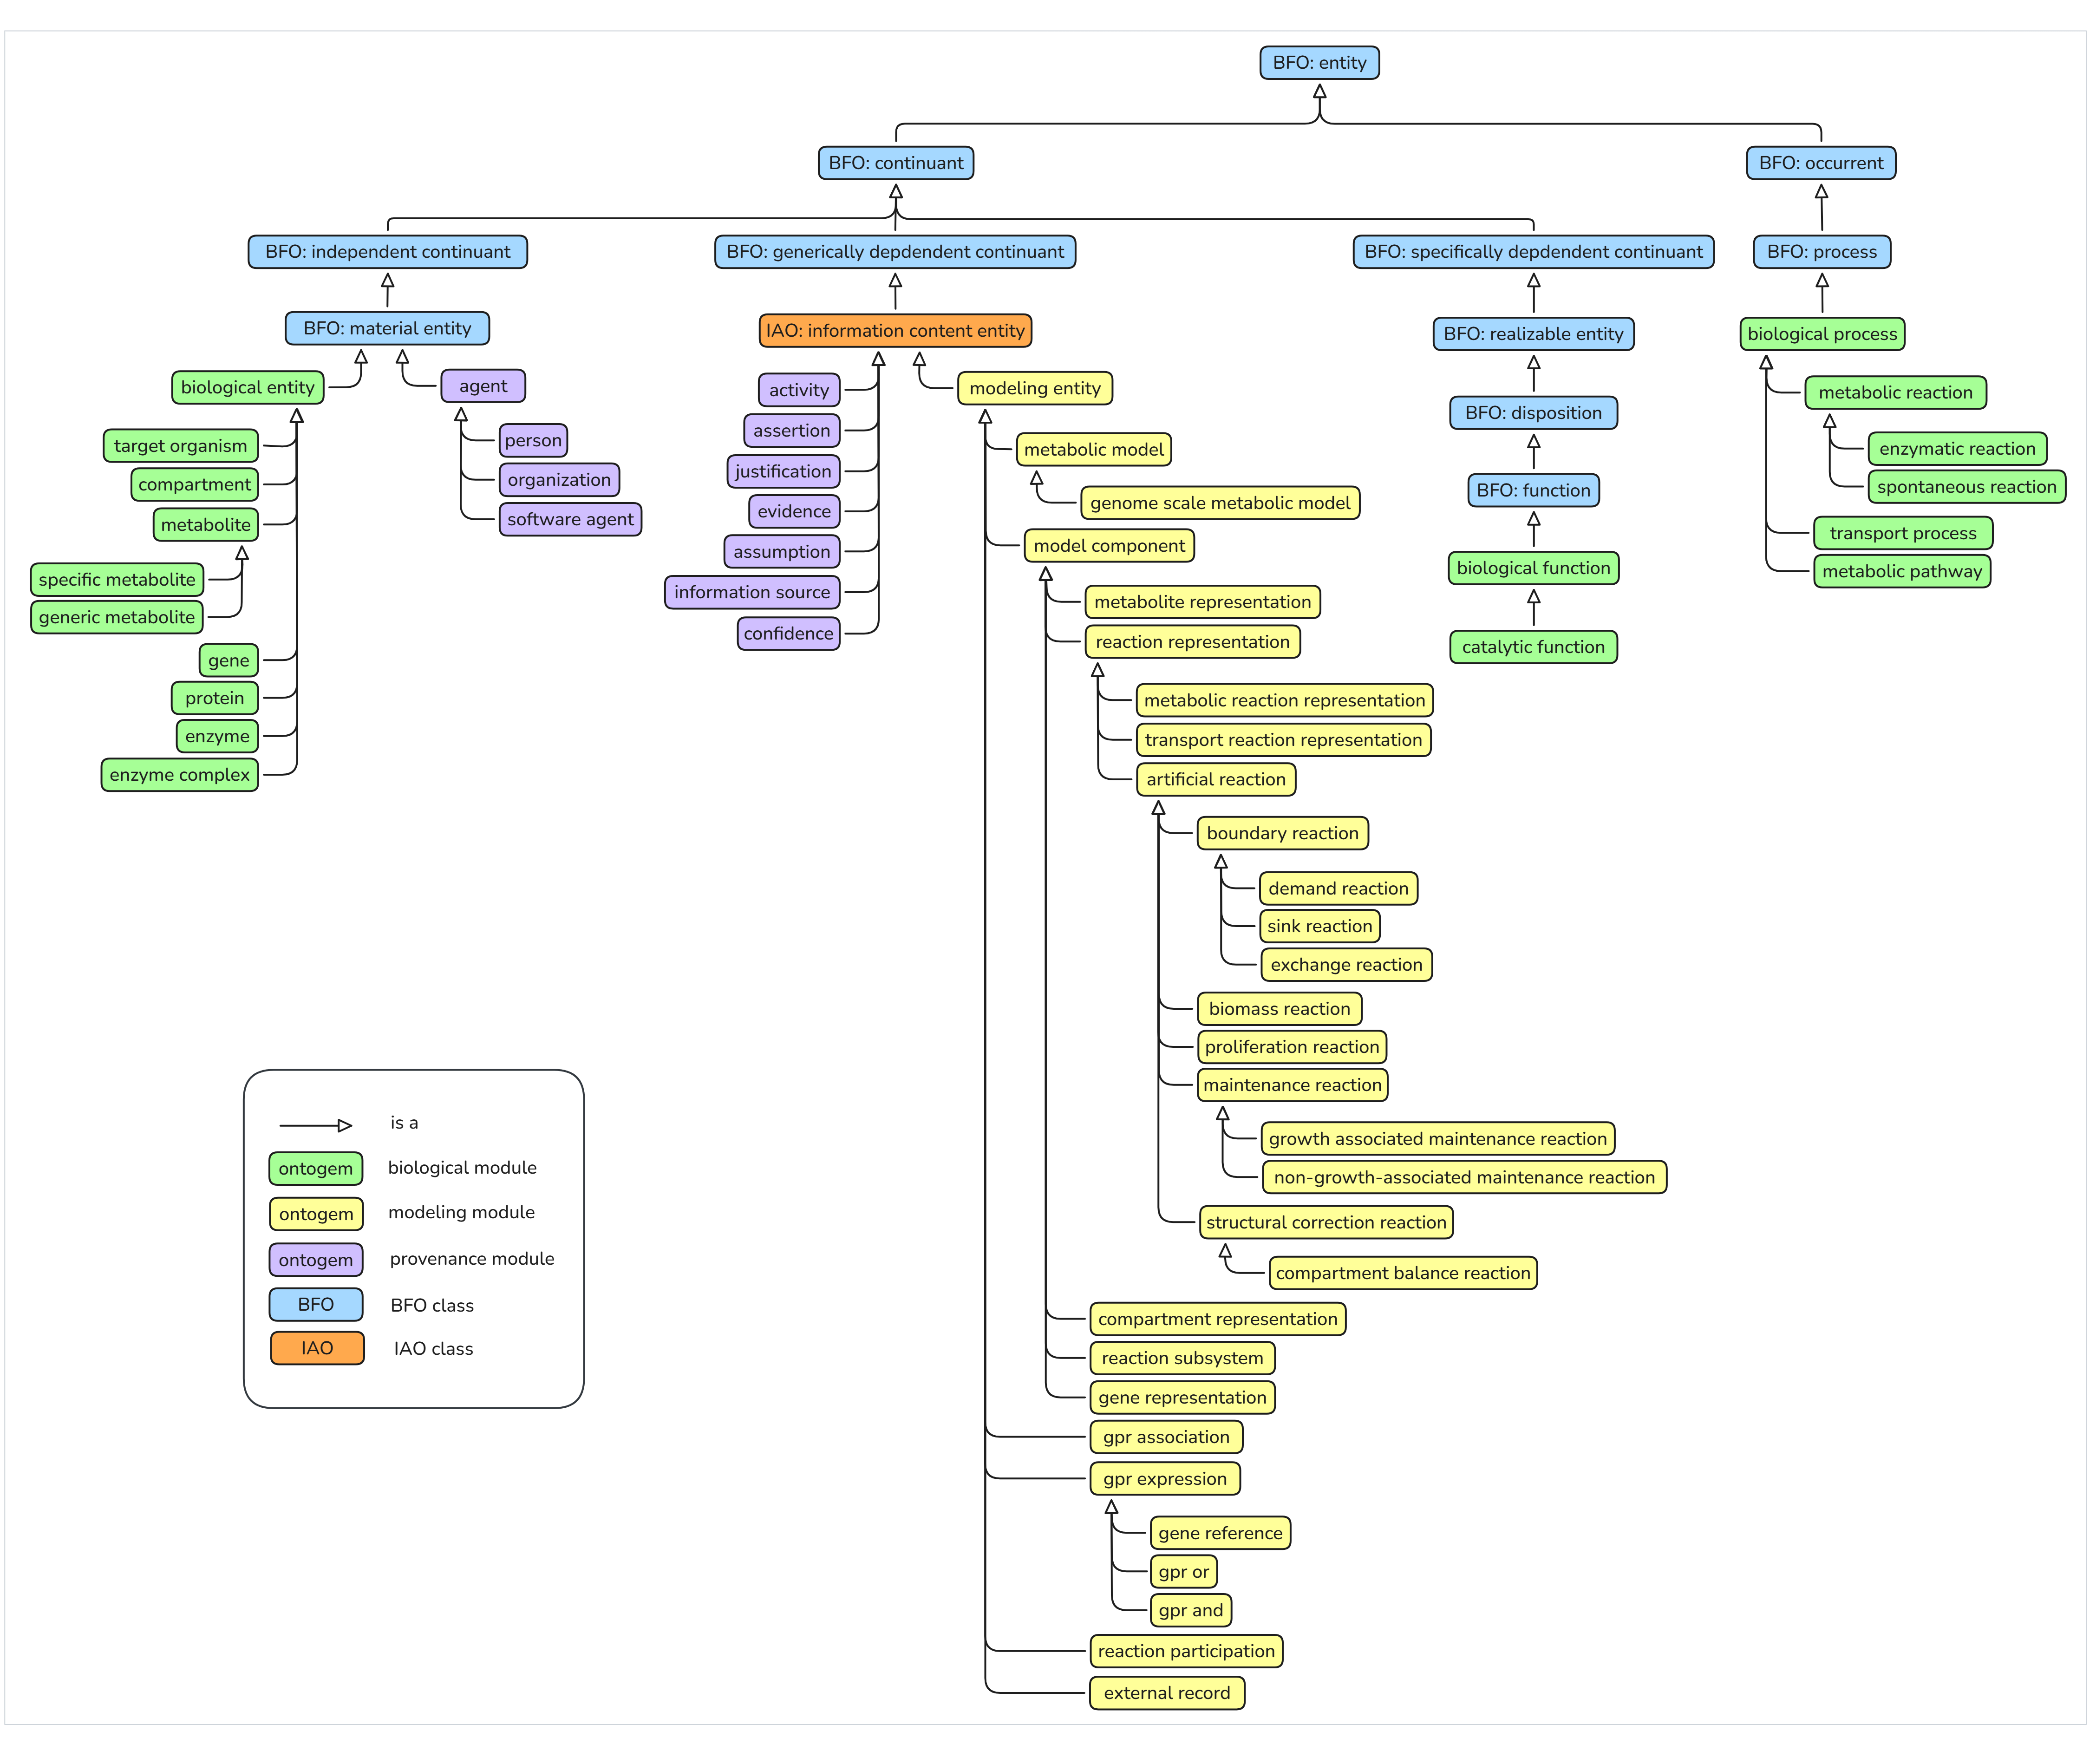
\includegraphics[width=0.70\linewidth]{img/new-relations-ontogem.png}
	\end{figure}
\end{frame}

 %  Principais desafios com RAG
\section{Perguntas de Pesquisa} % Seções são adicionadas para organizar sua apresentação em blocos discretos, todas as seções e subseções são automaticamente exibidas no índice como uma visão geral da apresentação, mas NÃO são exibidas como slides separados.

\begin{frame}
	\frametitle{Perguntas de Pesquisa}
	\begin{block}{RQ1 --- Ganho sobre o  RAG vetorial puro/\textit{baseline}}
		O uso do \textbf{OG-RAG} melhora as métricas de \textit{retrieval} (C-Rec, C-ERec) e de resposta (A-Sim, A-Corr) em relação ao \textit{baseline} de \textbf{busca vetorial pura}, na tarefa de perguntas sobre GEMs?
	\end{block}
	\begin{block}{RQ2 --- Impacto da curadoria humana na representação do conhecimento}
		A \textbf{curadoria humana da ontologia} por especialistas do domínio produz melhora significativa nessas métricas, quando comparada à  estrutura de representação simbólica de conhecimento gerada automaticamente do GraphRAG?
	\end{block}
\end{frame} % O que é o OG RAG
\section{Metodologia} % Seções são adicionadas para organizar sua apresentação em blocos discretos, todas as seções e subseções são automaticamente exibidas no índice como uma visão geral da apresentação, mas NÃO são exibidas como slides separados.

\begin{frame}
	\frametitle{Metodologia}
	\small
	
	\vfill
	\begin{columns}
		\begin{column}{0.60\textwidth}
			\begin{itemize}
				\item Confecção de um \textit{dataset} curado por especialistas sobre um GEM que tenha ampla cobertura no repositório BIGG e artigos científicos.
				\item Experimento comparativos de \textbf{três fases}, alterando-se \textbf{apenas o mecanismo de recuperação} entre elas , o que isola o efeito das \textbf{camadas simbólicas} sobre as métricas de qualidade do RAG.
				\item Ferramentas e LLMs \textit{open-source} serão utilizados.
				\item O \textit {framework open-source} RAGAS será utilizado para gerar as métricas de avaliação
			\end{itemize} 
		\end{column}
		\begin{column}{0.40\textwidth}
			\begin{figure}[H]
				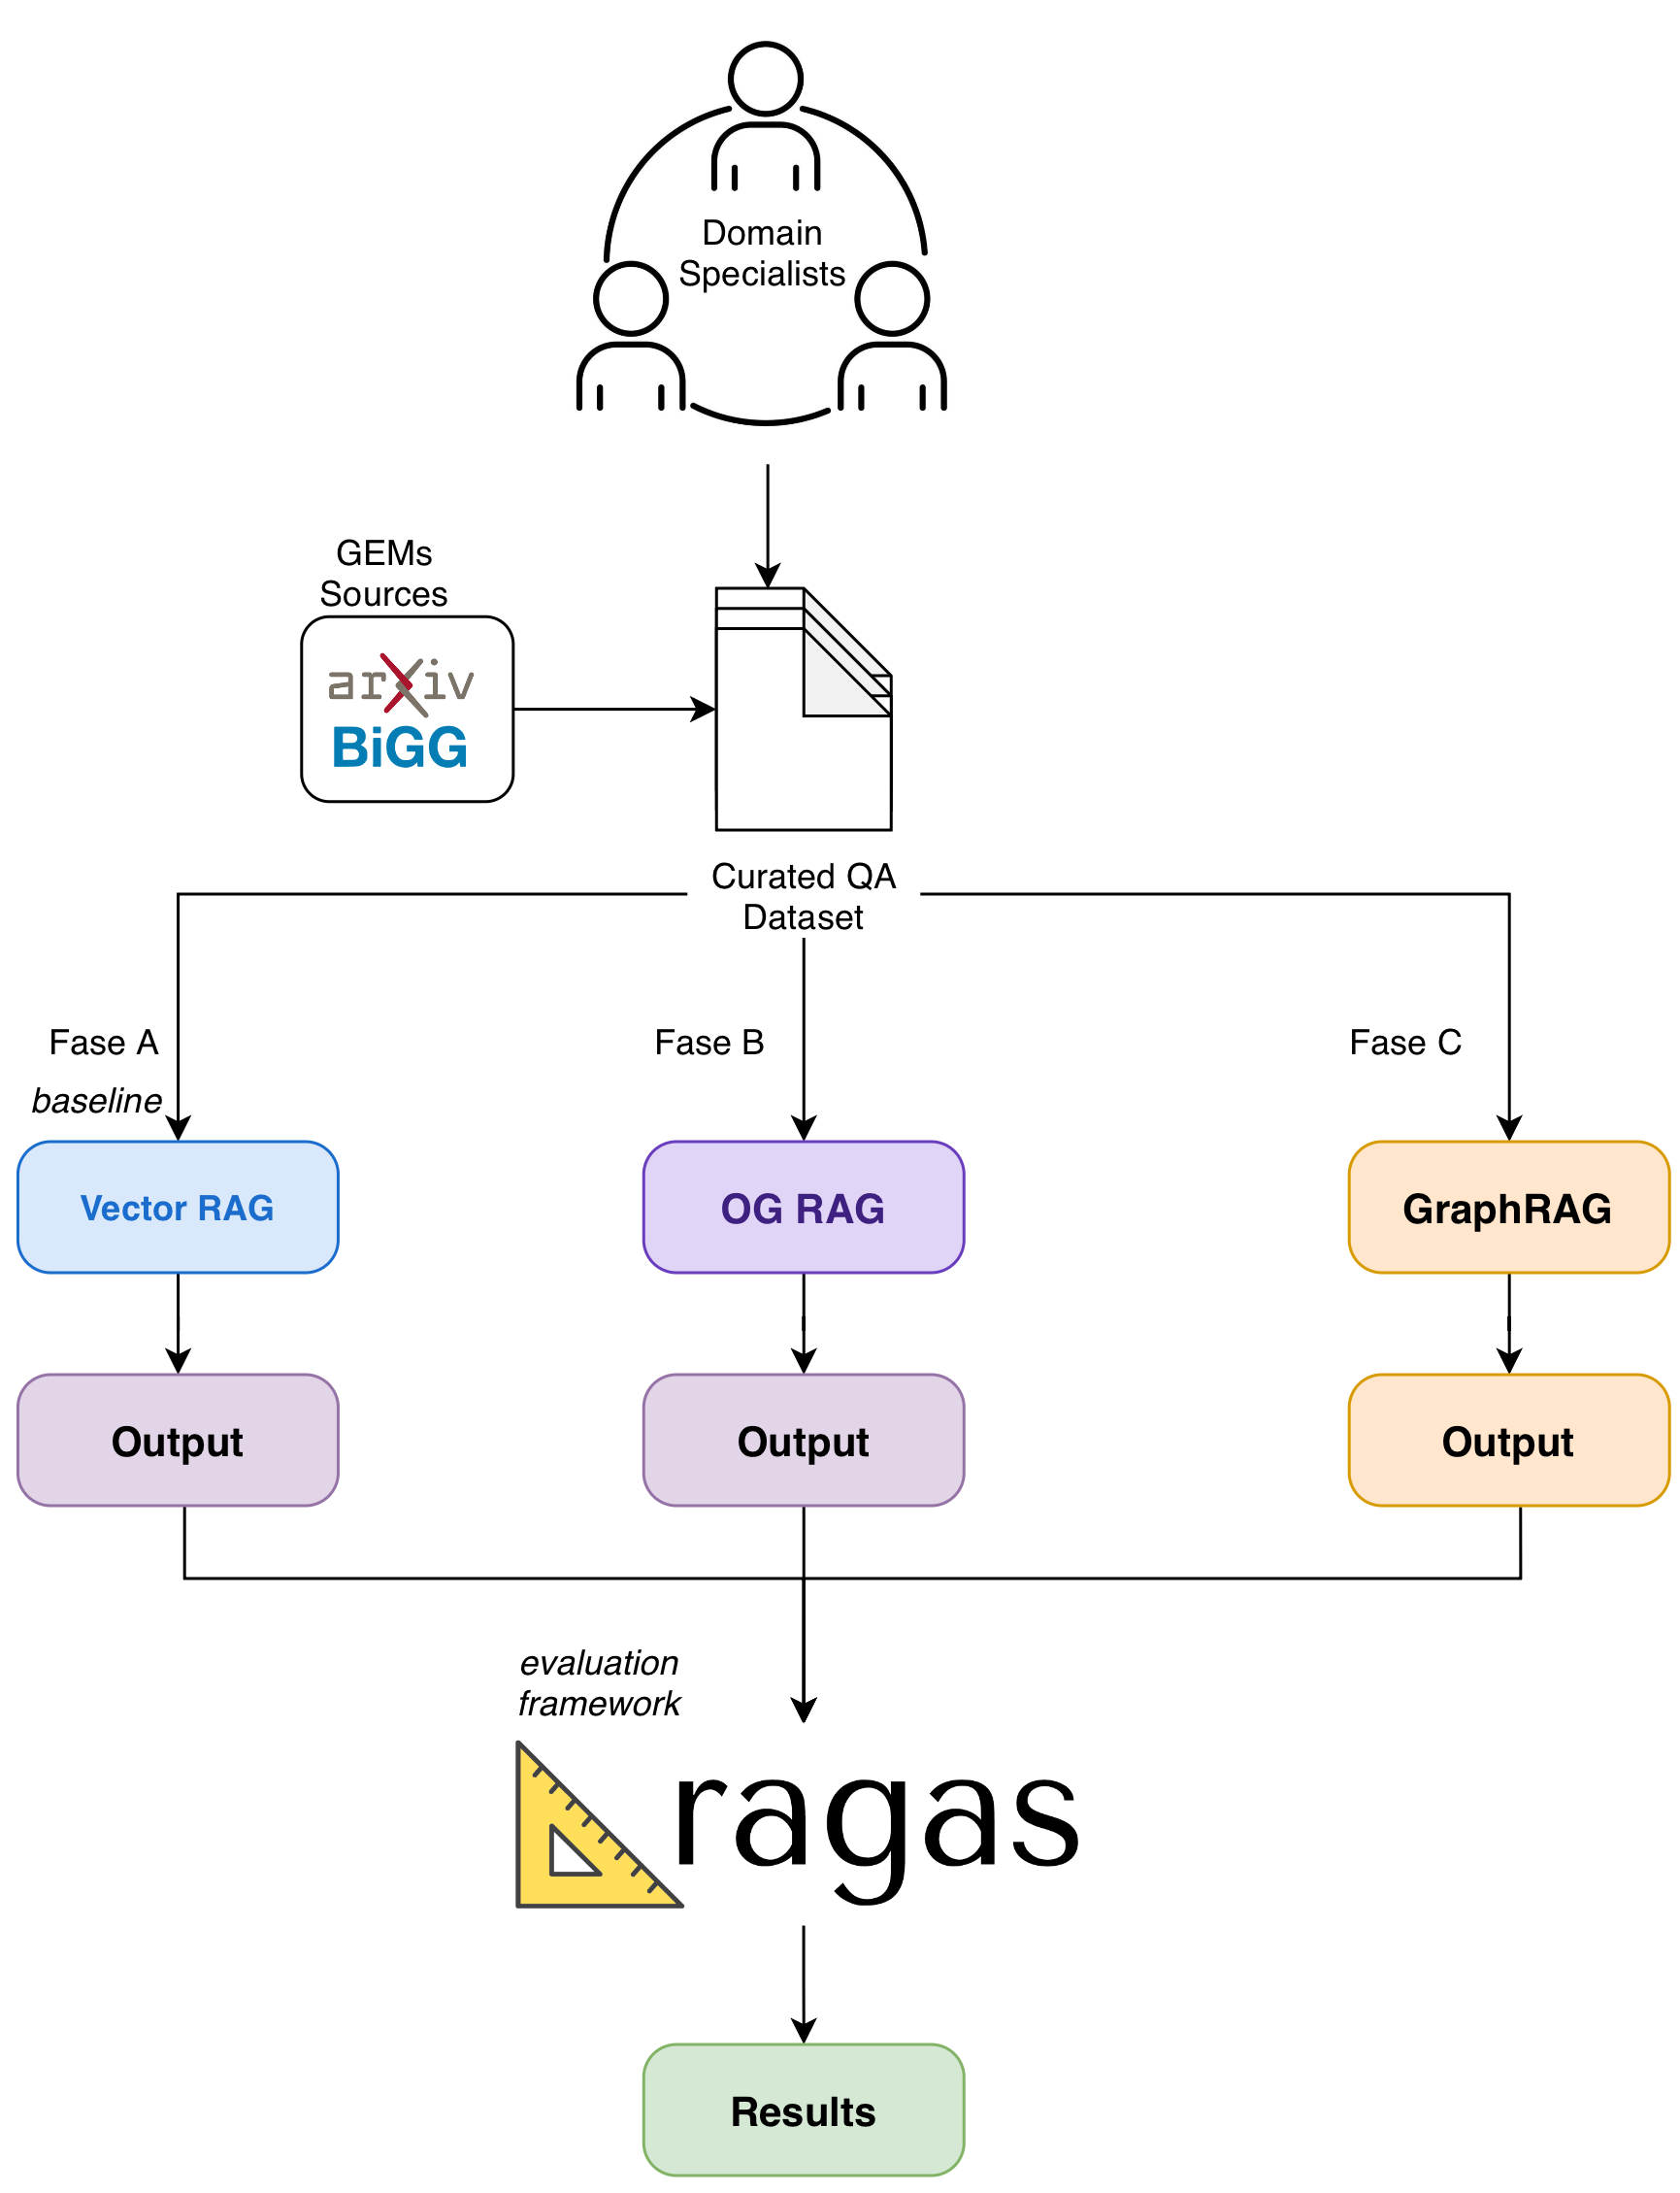
\includegraphics[width=\linewidth]{img/metodologia.png}
			\end{figure}
		\end{column}
	\end{columns}
\end{frame} % O que é o GraphRAG

\end{document}


